\chapter{Results}

All methods were implemented in the {\sc Psi4} electronic structure software package.
The parallelism in {\sc Psi4} relies on the shared memory programming model using OpenMP 
and carries out matrix multiplications using Intel's Math Kernel
Library. 

\section{Sparsity Screening}

We first demonstrate the performance of our Schwarz screening implementation 
by measuring the performance when computing the 3-center integrals, contracting the fitting metric,
and transforming the integrals into an MO basis.
The experiment employed an ideal sparse system: stacked benzenes. Execution times were recorded for each successive benzene
added to the stack, from one to ten benzenes, with each benzene spaced 5\AA\ apart.
Transformation time involved the wall time required to carry out the common occupied-virtual
transformation, as would be required by density-fitted MP2: 
\begin{align} 
(i b | Q) = (\lambda \sigma | Q) C_{\sigma i} C_{\lambda b} 
\end{align}

\noindent Where $i, j$ and $a, b$ denote occupied and virtual spaces, respectively. 
Algorithm 4 was implemented and used to carry out these transformations.
The cc-pVTZ and cc-pVTZ-jkfit basis sets were used for primary 
and auxiliary basis sets, respectively. The characteristics
of each system are listed in Table 2. The mask sparsity listed in Table 2 refers to the percentage of non-significant AO function pairs appearing in the sparsity mask.
The experiment was carried out using one node consisting of an Intel Core i7-5930K processor 
(6 cores at 3.50GHz) and 50GB DRAM. The results are plotted in Figure 2. Figure 2 (a), (b), (c), and (d) involve time to compute the 3-index integrals, contract the fitting metric,
perform the first transformation step: $(\mu \nu | Q)C_{i \mu} \rightarrow (i \nu | Q)$,
and total transform time, respectively.
Note that our novel contribution involves the application of the sparsity screening in the transformation step.

\begingroup
\begin{table}[H]
\centering
\renewcommand{\baselinestretch}{1}
\caption{Characteristics of benzene stack systems. $N$ and $N_{aux}$ refer to the number of primary and auxiliary basis functions, respectively.
 Mask sparsity refers to the percentage of significant AO function pairs in the sparsity mask. Mask sparsity increases with additional benzenes added to the stack.}
\begin{tabular}{l ccc}
\multicolumn{1}{l}{\textbf{Benzenes}} &
\multicolumn{1}{c}{\textbf{$N$}} &
\multicolumn{1}{c}{\textbf{$N_{aux}$}} &
\multicolumn{1}{c}{\textbf{Mask Sparsity (\%)}} \\
\hline
1        & 264  & 654       & 2.6              \\ 
2        & 528  & 1308      & 24.7             \\ 
3        & 792  & 1962      & 43.6             \\ 
4        & 1056 & 2616      & 55.3             \\ 
5        & 1320 & 3270      & 63.1             \\ 
6        & 1584 & 3924      & 68.6             \\ 
7        & 1848 & 4578      & 72.7             \\ 
8        & 2112 & 5232      & 75.9             \\ 
9        & 2376 & 5886      & 78.4             \\ 
10       & 2640 & 6540      & 80.4             \\ 
\end{tabular}
\end{table}
\endgroup

\begin{figure}[H]
  \centering
  \subfloat[]{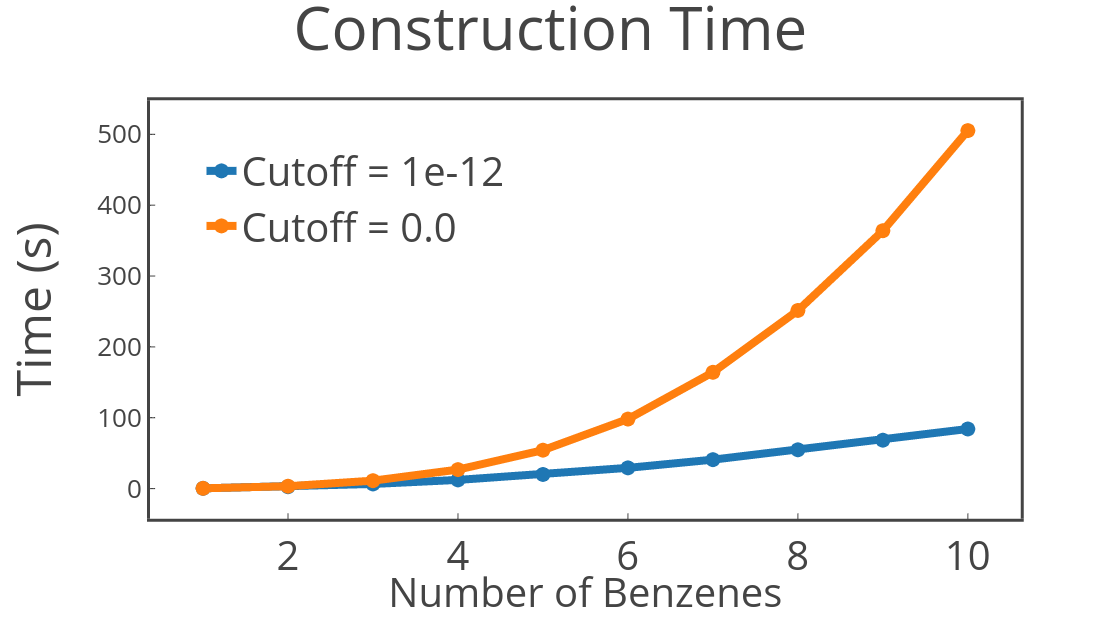
\includegraphics[width=0.5\textwidth]{figures/sparsity_plots/construction_wall.png}\label{fig:f1}}
  \hfill
  \subfloat[]{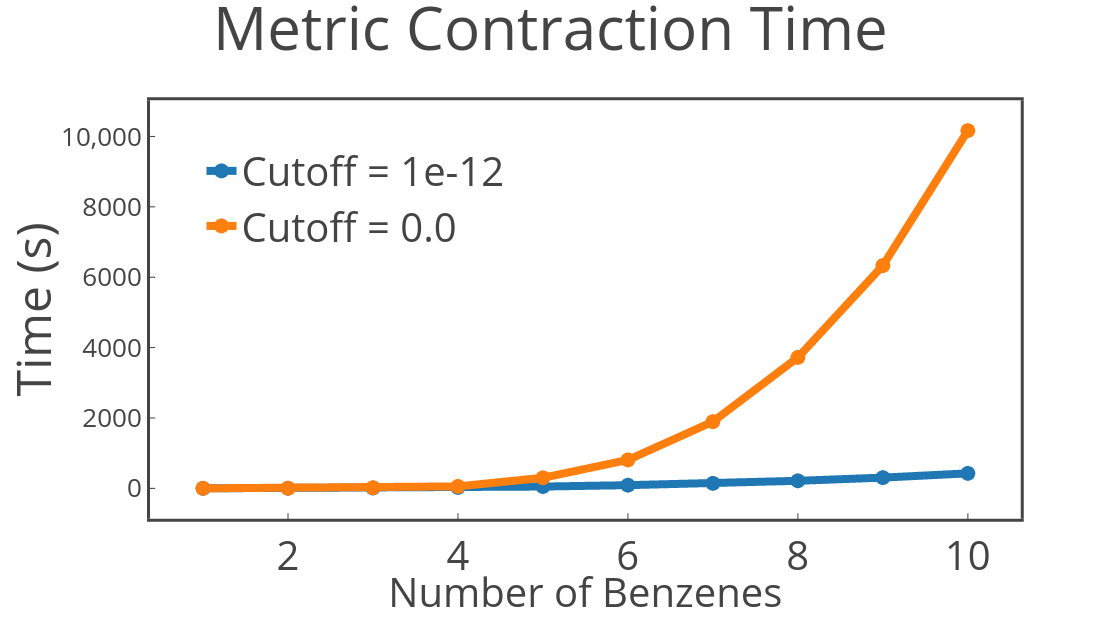
\includegraphics[width=0.5\textwidth]{figures/sparsity_plots/metric_contraction.png}\label{fig:f1}}
  \hfill \\
  \subfloat[]{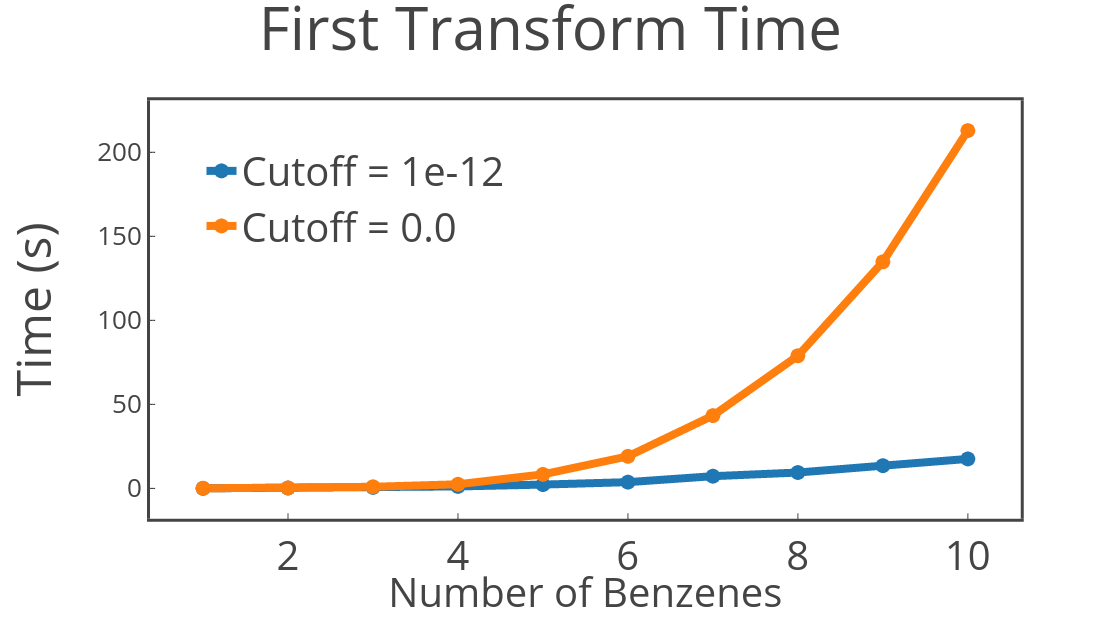
\includegraphics[width=0.5\textwidth]{figures/sparsity_plots/first_transform_wall.png}\label{fig:f1}}
  \hfill
  \subfloat[]{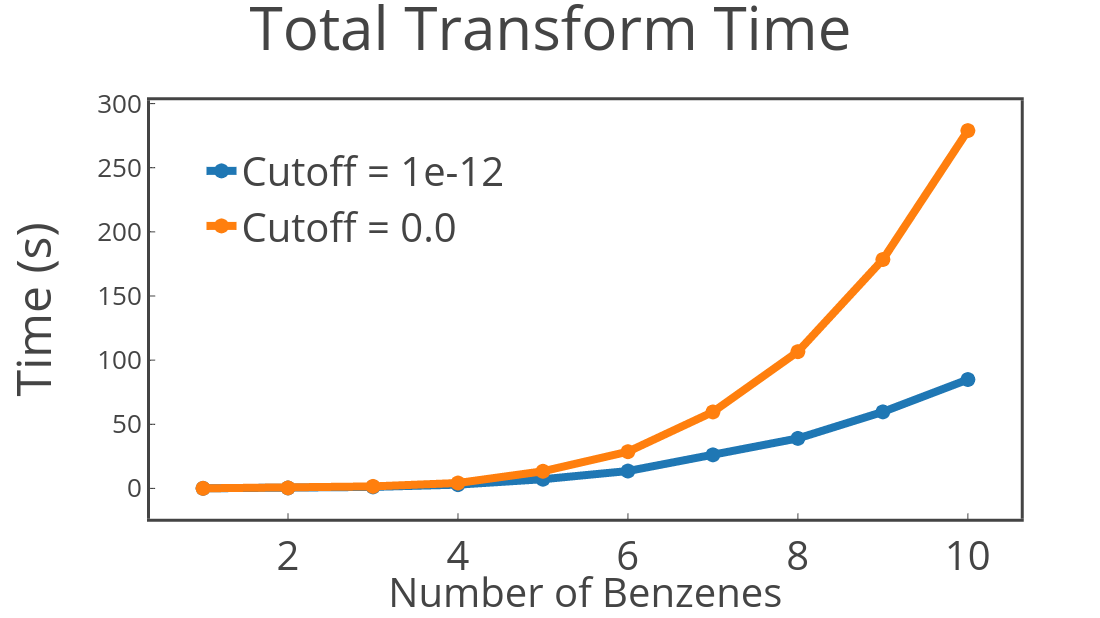
\includegraphics[width=0.5\textwidth]{figures/sparsity_plots/total_transform_wall.png}\label{fig:f2}}
  \caption{Comparison of execution times using sparsity screening (blue) against no sparsity screening (orange).  Execution time is plotted against number of benzenes
 in a benzene stack from one to ten benzenes. Transformations involved computing $(ib|Q)$, where $i$ and $b$ denote occupied and virtual indices, respectively.
 Cutoff refers to the Schwarz screening threshold. (a) Computing the integrals. (b) Contracting AO integrals with the fitting metric. 
(c) first transformation times only. (d) total transformation times.}
\end{figure}

\begingroup
\begin{table}[H]
\centering
\renewcommand{\baselinestretch}{1}
\caption{Speedups obtained from sparsity screening at ten benzenes from data in Figure 2.}
\begin{tabular}{l c}
\multicolumn{1}{l}{\textbf{Operation}} &
\multicolumn{1}{c}{\textbf{Speedup at 10 benzenes}} \\ 
\hline
Construction          & 10.6  \\          
Metric Contraction    & 37.8  \\          
First Transformation  & 25.8  \\          
Total Transformation  & 5.5  \\          
\end{tabular}
\end{table}
\endgroup


Clearly, Figure 2 reveals significant time reductions for all procedures measured.
Table 3 reinforces that operations with higher complexity scaling have the largest time
reduction, with the caveat that total transformation time includes portions without sparsity utilization.
In the integral computations (Figure 2 (a)), we construct the sparse integrals using
function screening; however, we still compute them in shell triplets for effeciency.
Therefore the acquired speedup is slightly less dramatic compared to the metric contraction and
transformation procedures (Figure 2 (b) and (c), respectively) due to select functions being 
screened in cases where the entire shell is not screened. 
Note that the metric contraction is by far the most expensive operation, which should in one part
highlight the boon of sparsity utilization and in another part
illustrate the pertinence of our workflow investigation later in this paper.
Last, our proposal outlined in Algorithm 2 for applying sparsity screening to integral transformations
is proven viable by Figure 2 (c).  Note that significant reductions are obtained for the
first transformation; however, the sparsity thereafter is unrelated to the initial sparsity
mask. With sparsity utilization, the first step scales as $\mathcal{O}(N_{aux}N_{AO}^{1-2}p)$,
whereas the second transformation step will still scale as $\mathcal{O}(N_{aux}N_pN_q)$.
In this work we have not gone on to consider sparsity of the MO indices, which would 
typically require transformation to local orbitals.


\section{Parallel Scaling of Transformations}

To measure parallel scaling, we performed integral transformations for the boron catalyst system shown in Figure 3. 
We varied the problem size by adjusting the $\zeta$ level for the Dunning basis sets with $\zeta$ = D, T, Q.
The characteristics of these systems are included in Table 4. Note that while parallel scaling typically improves
for larger systems (i.e. due to larger workloads),
this is not gauranteed in a sparsity regime. Larger systems may contain more sparsity;
more sparsity will result in more striding, copying, and irregular sizing,
which will hinder parallel scaling. Nonetheless, our method outlined in Algorithm 2 is designed to utilize sparsity while also
obtaining maximum parallel efficiency. 

\begin{figure}[H] 
\centering
\includegraphics[width=80mm]{geometries/boron_catalyst.png} \caption{Transition state for organoboron addition to trifluooroacetone. Taken from Ref. \cite{Lec:2016:768}} 
\label{fig:databases} \end{figure}

\begingroup
\begin{table}[H]
\centering
\renewcommand{\baselinestretch}{1}
\caption{Characteristics of organoboron catalyst.
$N$ and $N_{aux}$ refer to the number of primary and auxiliary basis functions, respectively.
Mask sparsity refers to the percentage of significant AO function pairs in the sparsity mask.}
\begin{tabular}{l ccc}
\multicolumn{1}{l}{\textbf{Basis}} &
\multicolumn{1}{c}{\textbf{$N$}} &
\multicolumn{1}{c}{\textbf{$N_{aux}$}} &
\multicolumn{1}{c}{\textbf{Mask Sparsity (\%)}} \\
\hline
cc-pVDZ   & 671  & 3277 & 29.6 \\          
cc-pVTZ   & 1566 & 3856 & 41.1 \\          
cc-pVQZ   & 3040 & 5593 & 50.2 \\          
\end{tabular}
\end{table}
\endgroup

\noindent For each system, we performed the three common transformations:

\begin{align} 
(i j | Q) = (\lambda \sigma | Q) C_{\sigma i} C_{\lambda j} \\
(i b | Q) = (\lambda \sigma | Q) C_{\sigma i} C_{\lambda b} \\
(a b | Q) = (\lambda \sigma | Q) C_{\sigma a} C_{\lambda b} 
\end{align}

\noindent The experiment was carried out using one node consisting of an Intel Xeon E5-2630 processor 
(10 cores at 2.20GHz) and 24GB DRAM. Figure 4 includes plots of both speedups and execution times for each system.

\begin{figure}[H]
  \centering
  \subfloat[]{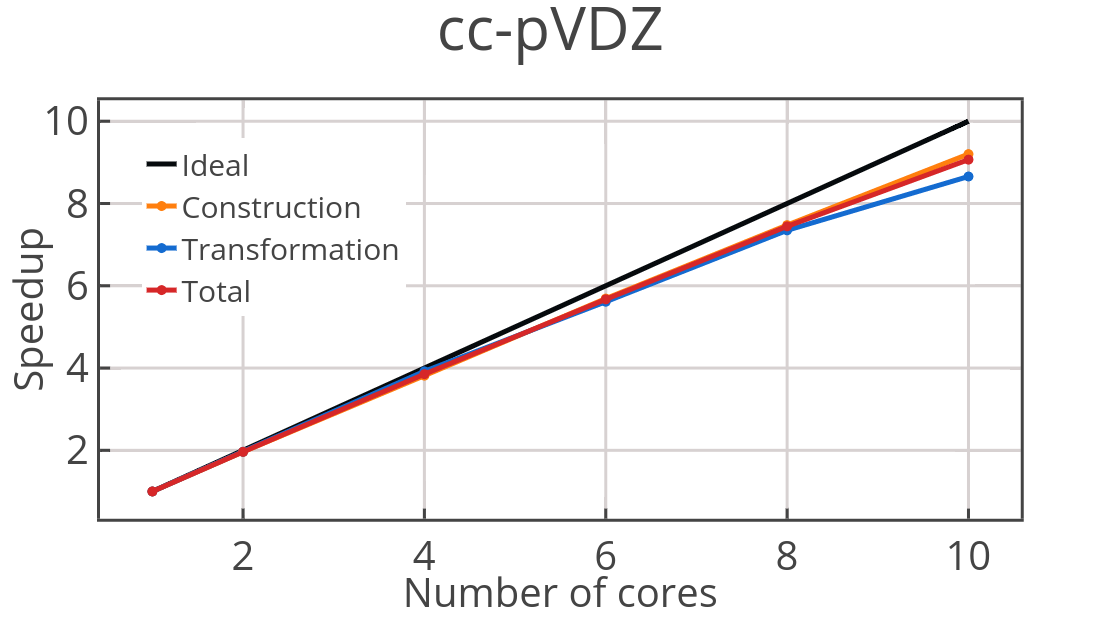
\includegraphics[width=0.5\textwidth]{figures/parallel_scaling_plots/speedup-cc-pVDZ.png}\label{fig:f1}}
  \hfill
  \subfloat[]{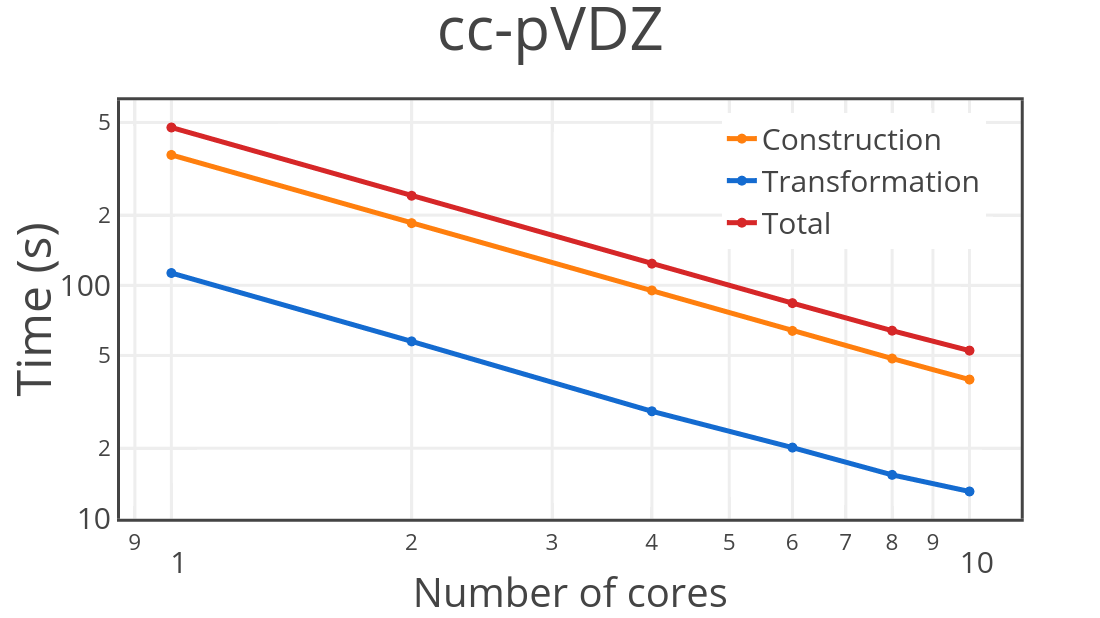
\includegraphics[width=0.5\textwidth]{figures/parallel_scaling_plots/times-cc-pVDZ.png}\label{fig:f2}}
  \hfill
  \subfloat[]{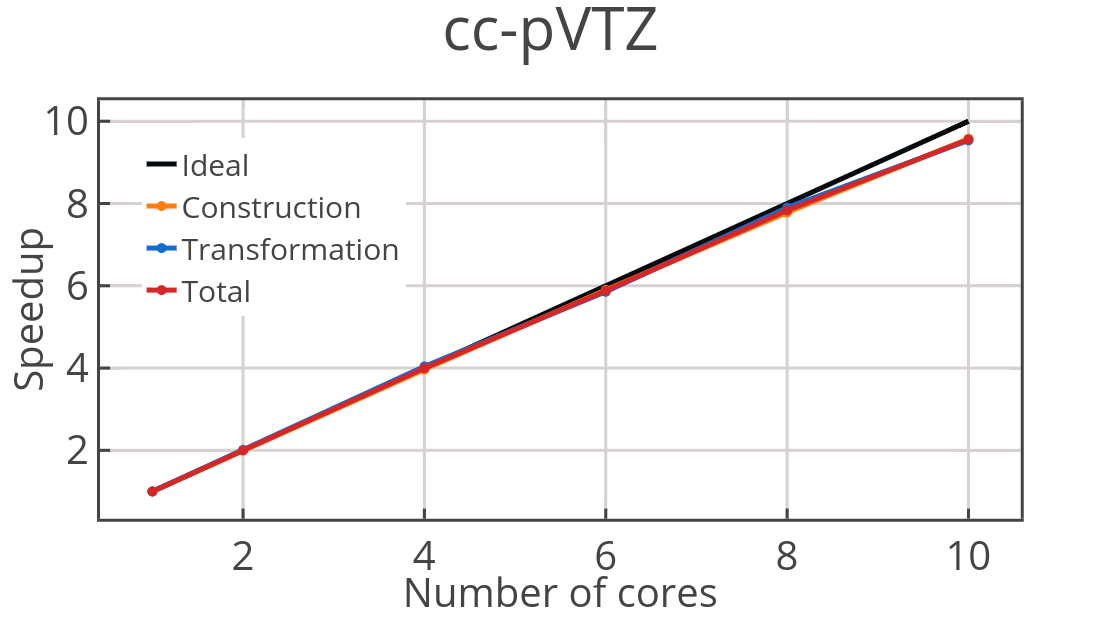
\includegraphics[width=0.5\textwidth]{figures/parallel_scaling_plots/speedup-cc-pVTZ.png}\label{fig:f1}}
  \hfill
  \subfloat[]{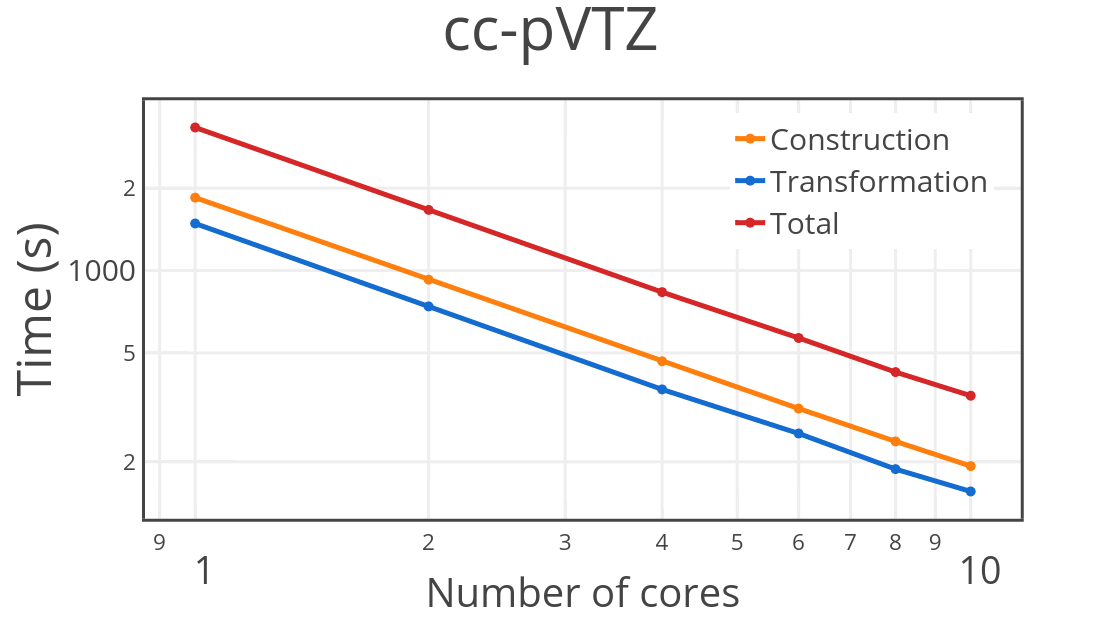
\includegraphics[width=0.5\textwidth]{figures/parallel_scaling_plots/times-cc-pVTZ.png}\label{fig:f2}}
  \hfill
  \subfloat[]{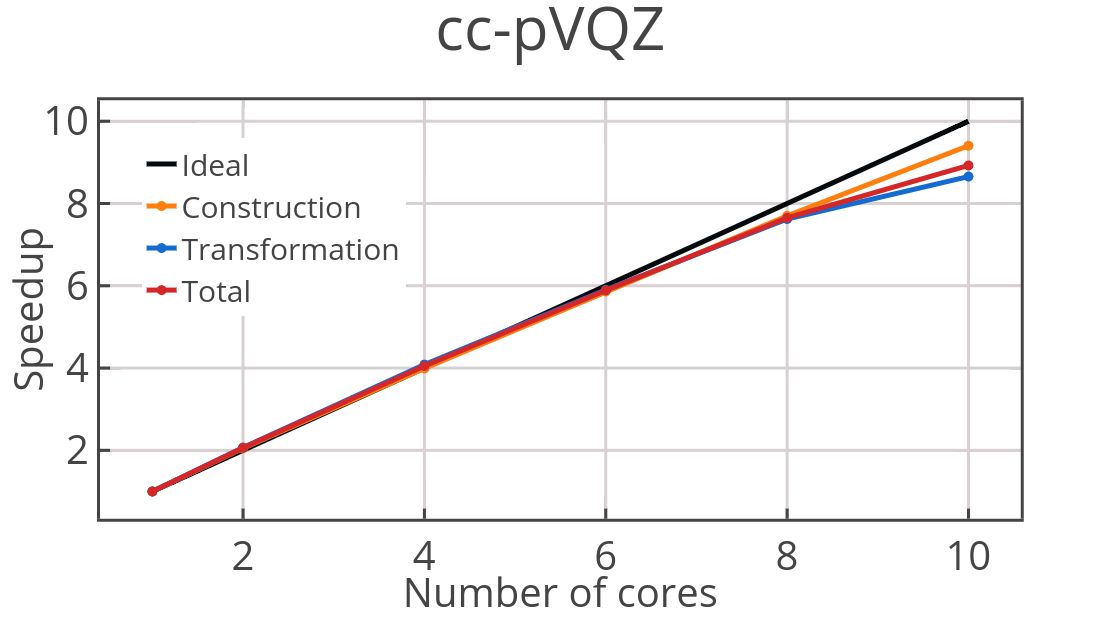
\includegraphics[width=0.5\textwidth]{figures/parallel_scaling_plots/speedup-cc-pVQZ.png}\label{fig:f1}}
  \hfill
  \subfloat[]{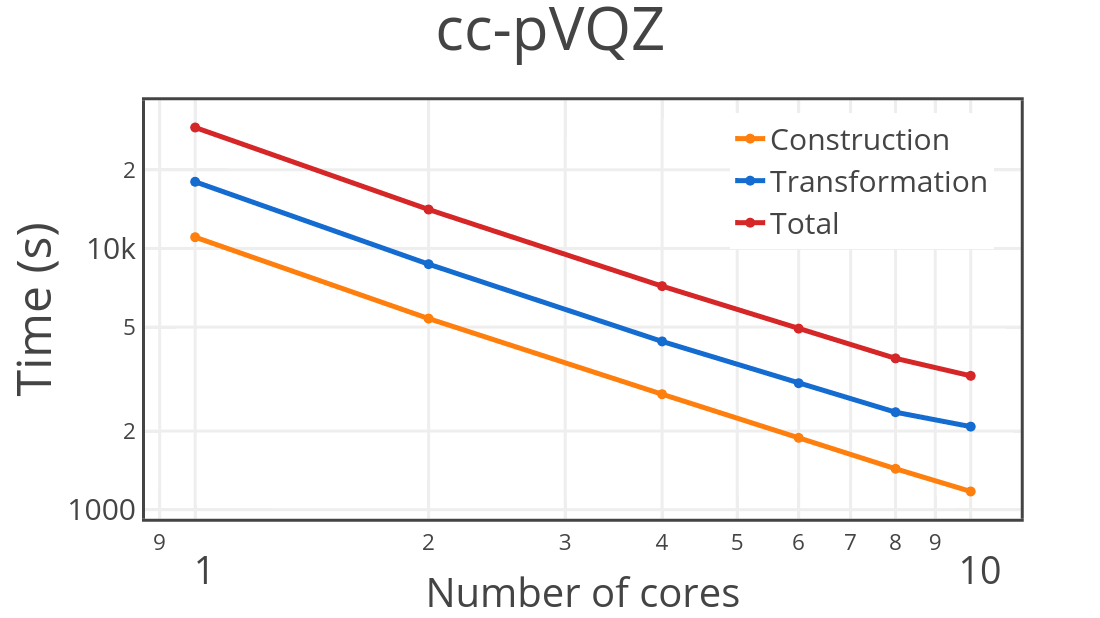
\includegraphics[width=0.5\textwidth]{figures/parallel_scaling_plots/times-cc-pVQZ.png}\label{fig:f2}}
  \hfill
  \caption{Speedup and execution time plots obtained using our optimized memory layout from Section 3 for sparsity screened 3-center integrals. 
 Execution times involve computing three common transformations: $(ij|Q)$, $(ib|Q)$, and $(ab|Q)$,
 where $i,j$ and $a,b$ denote occupied and virtual indices, respectively. Graphs (a), (c), and (e) include speedups for constructing the integrals (orange),
 transforming (blue), total time (red), and ideal (black). Graphs (b), (d), and (f) plot total execution times. Problem sizes were increased by increasing basis set size
 using cc-pVXZ, X = D,T,Q.}
\end{figure}

At ten cores, speedups for total computation time were recorded as 9.09, 9.56, and 8.93 for $\zeta = $ D, T, Q, 
respectively. The improvement in scaling between $\zeta = $ D to $\zeta = $ T
may be attributed to larger system sizes. The sizes of the sparsity screened AO integrals were 10.38GB and 55.70GB 
for these systems, respectively. In the latter case,
the 24GB of memory at the compute node was fully used and work for each thread was increased to maximal levels. Conversely, 
when the system size was increased again using
$\zeta = $ Q, the memory contraint did not allow for further increase in work per thread. 
The hindrance in scaling from $\zeta = $ T to $\zeta = $ Q is explained by the workload inbalance incurred by
the increase in sparsity. 


\section{Context Dependent Workflows}

\subsection{Performace Crossover Through Number of Iterations}
 In this section, we reveal the contexts in which either the Store or Direct algorithms are superior. First, we analyzed performance when applying either algorithm
 to carry out each of the three common integral transformations: $(Q|ij)$, $(Q|ib)$, and $(Q|ab)$. Doing so reveals the crossover in computational complexity that occurs between the two
 algorithms. For few transformations, the Direct algorithm will be superior as it benefits from the speedups given
 in Table 1. However, if many transformations occur, we propose the Store algorithm will become superior as it avoids the costly metric contraction for each transformation.
 
We applied both algorithms to each transformation using the
same boron catalyst system in Section 6.2. To reveal the crossover in computational work between the two algorithms, 
the execution times to carry out one to ten transformations were recorded. To reveal additional trends, we varied the
system size by adjusting the basis set size using $\zeta$ = D, T, Q. The characteristics of these systems are described in Table 5.
The experiments were carried out using one node consisting of an Intel Core i7-5930K processor
(6 cores at 3.50GHz) and 50GB DRAM. The results are plotted in Figure 5.
 
\begingroup
\begin{table}[H]
\centering
\renewcommand{\baselinestretch}{1}
\caption{Characteristics of organoboron catalyst systems across the cc-pVDZ, cc-pVTZ, and cc-pVQZ basis sets.}
\begin{tabular}{l cccc}
\multicolumn{1}{l}{\textbf{Basis}} &
\multicolumn{1}{c}{\textbf{$N$}} &
\multicolumn{1}{c}{\textbf{$N_{aux}$}} &
\multicolumn{1}{c}{\textbf{$N_{occ}$}} &
\multicolumn{1}{c}{\textbf{$N_{virt}$}} \\
\hline
cc-pVDZ   & 671  & 3277      & 129       & 542        \\ 
cc-pVTZ   & 1566 & 3856      & 129       & 1437       \\ 
cc-pVQZ   & 3040 & 5593      & 129       & 2911       \\ 
\end{tabular}
\end{table}
\endgroup

\begin{figure}[H]
  \captionsetup[subfigure]{labelformat=empty}
  \centering
  \subfloat[]{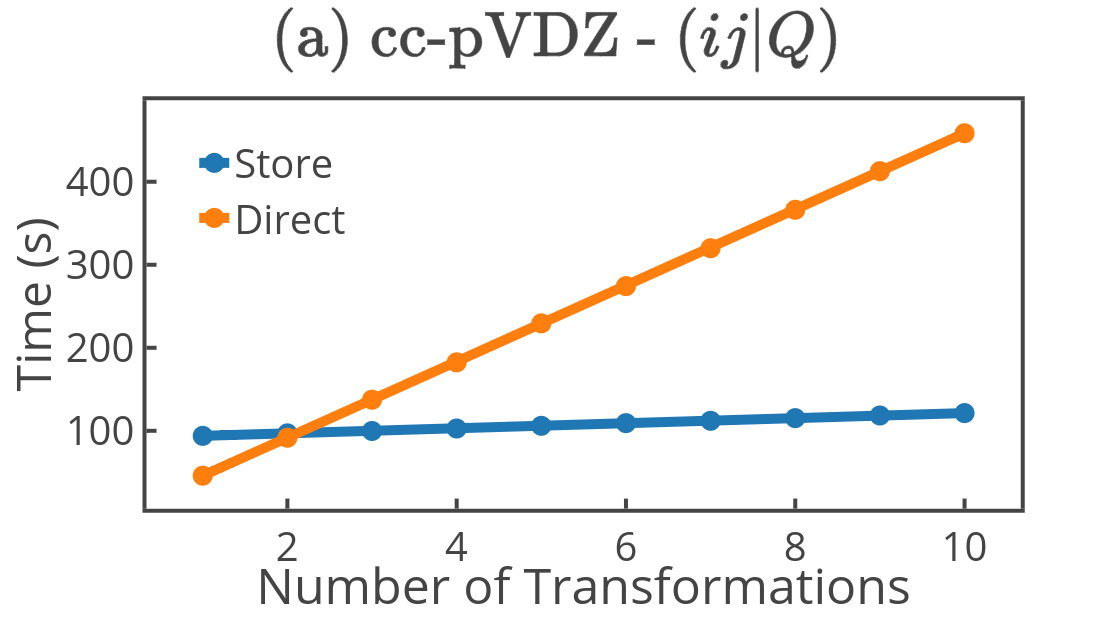
\includegraphics[width=0.35\textwidth]{figures/workflow_plots/input1-cc-pVDZ.png}}
  %\hfill
  \subfloat[]{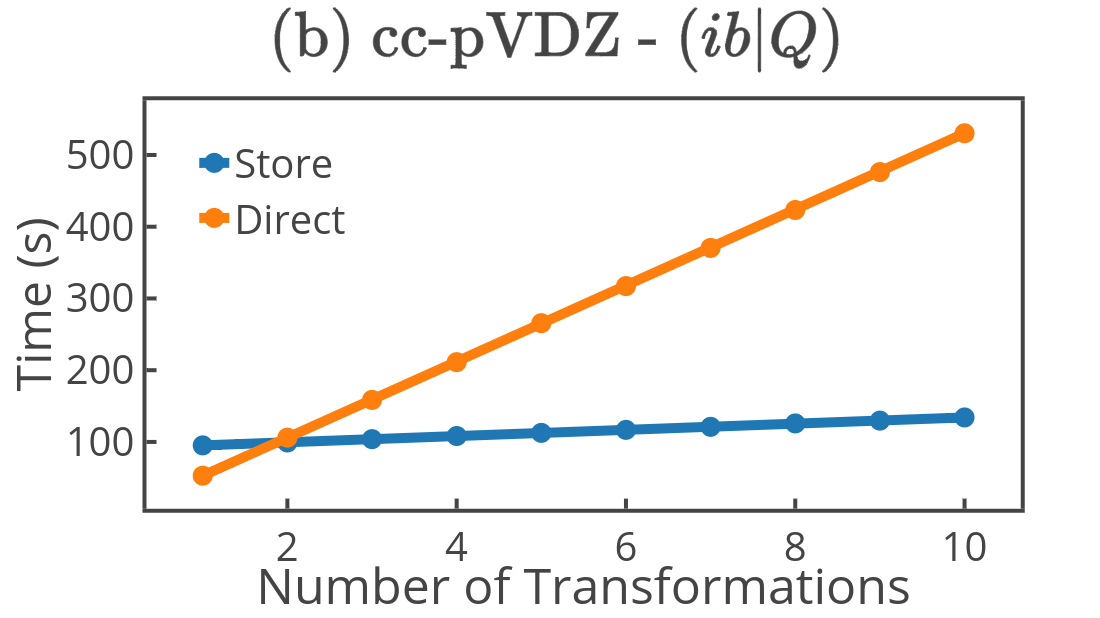
\includegraphics[width=0.35\textwidth]{figures/workflow_plots/input2-cc-pVDZ.png}}
  %\hfill
  \subfloat[]{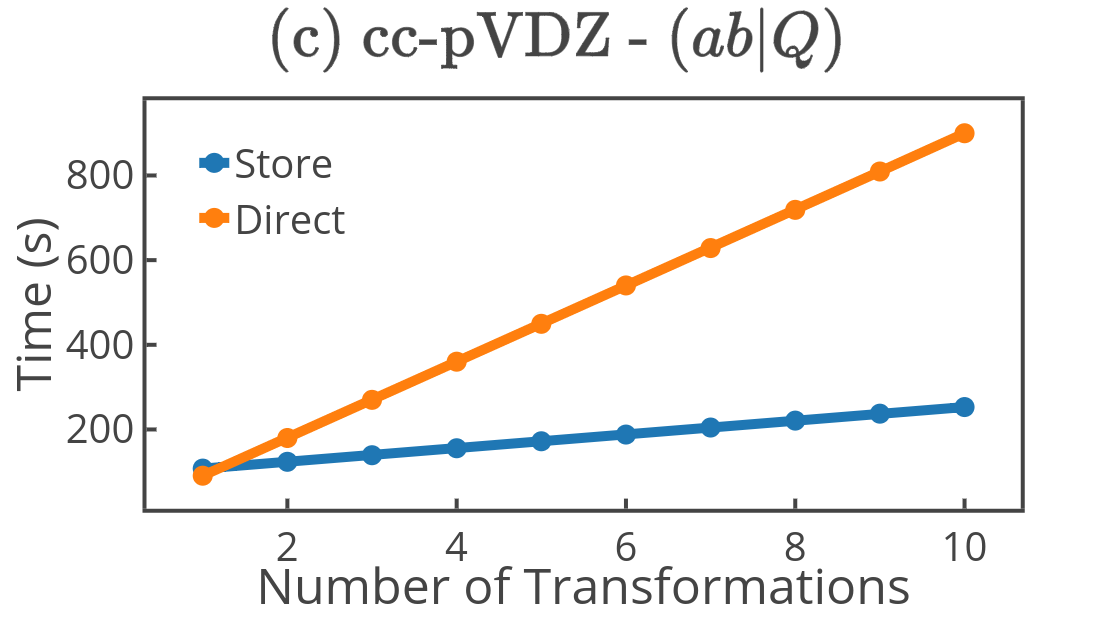
\includegraphics[width=0.35\textwidth]{figures/workflow_plots/input3-cc-pVDZ.png}}\\[-4ex]
  \hfill
  \subfloat[]{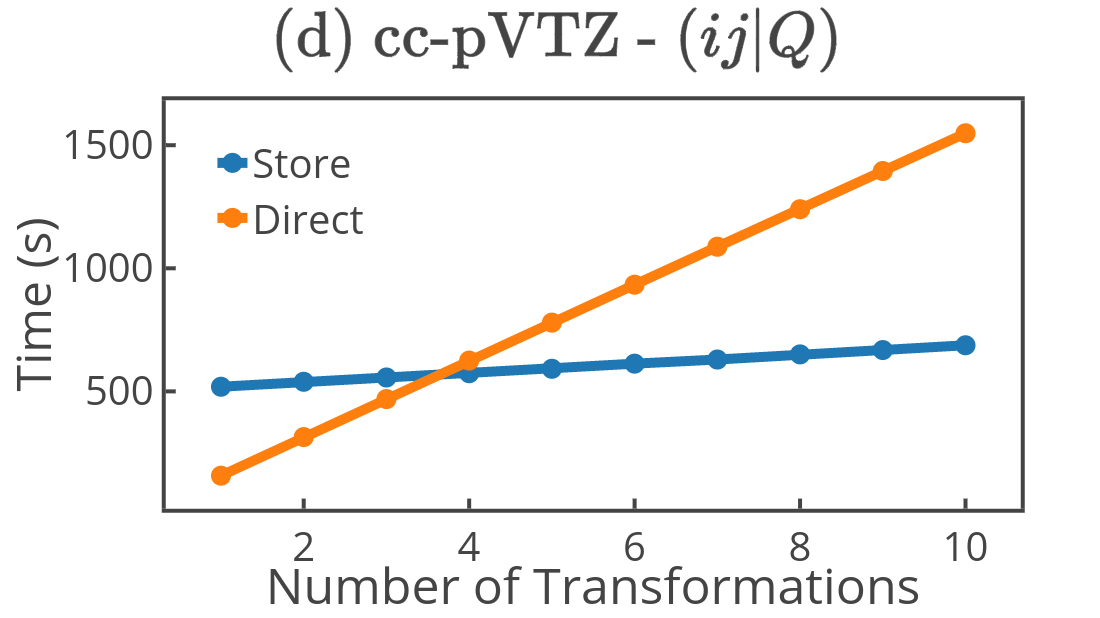
\includegraphics[width=0.35\textwidth]{figures/workflow_plots/input1-cc-pVTZ.png}}
  %\hfill
  \subfloat[]{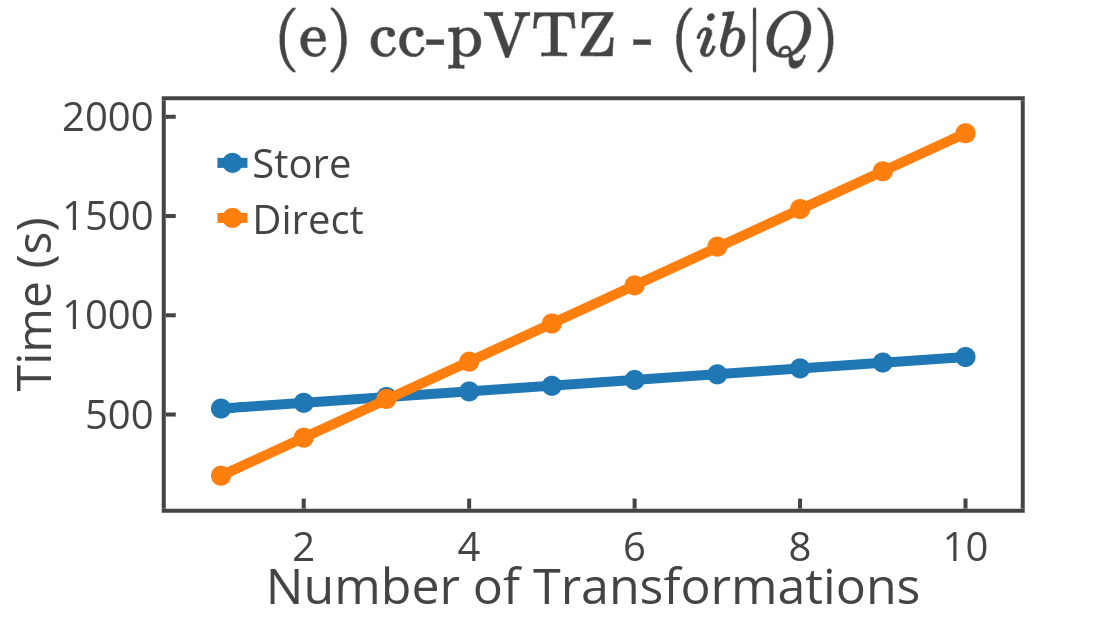
\includegraphics[width=0.35\textwidth]{figures/workflow_plots/input2-cc-pVTZ.png}}
  %\hfill
  \subfloat[]{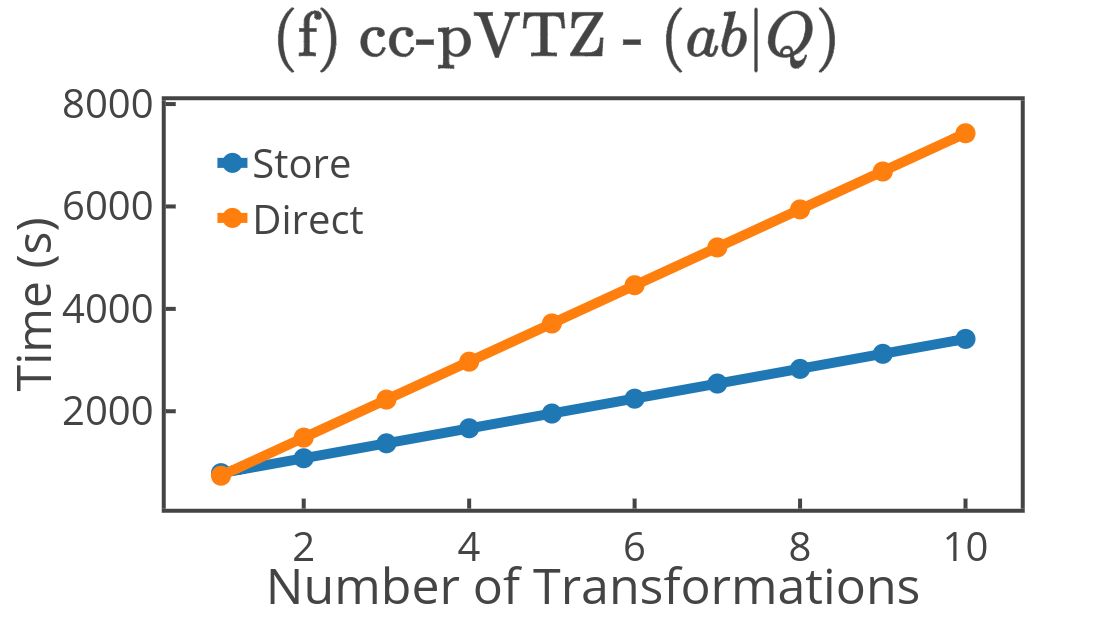
\includegraphics[width=0.35\textwidth]{figures/workflow_plots/input3-cc-pVTZ.png}}\\[-4ex]
  \hfill
  \subfloat[]{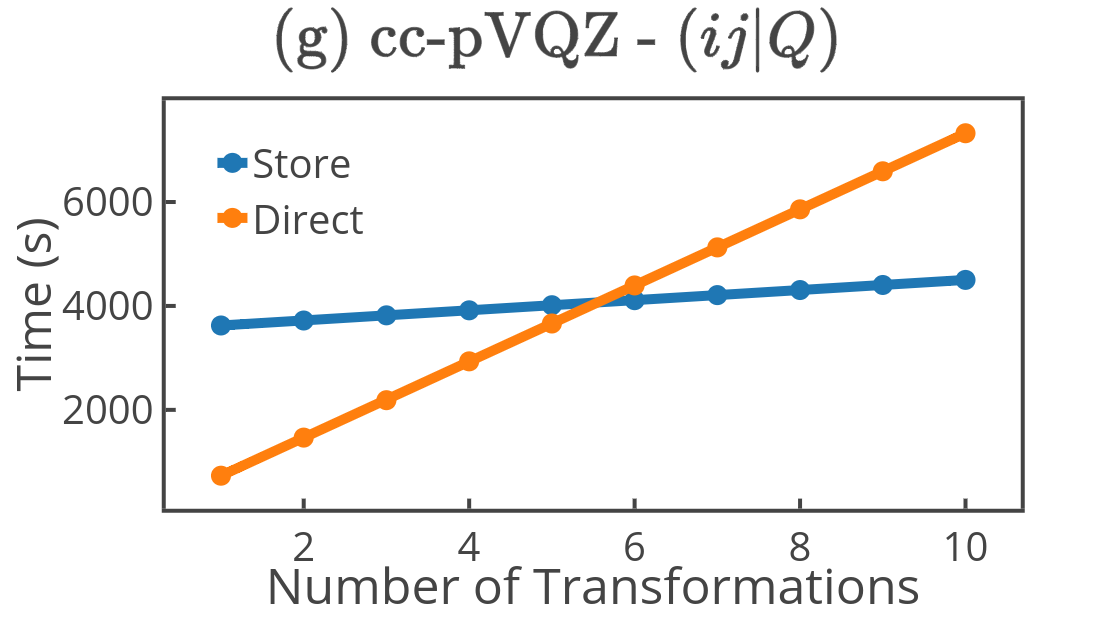
\includegraphics[width=0.35\textwidth]{figures/workflow_plots/input1-cc-pVQZ.png}}
  %\hfill
  \subfloat[]{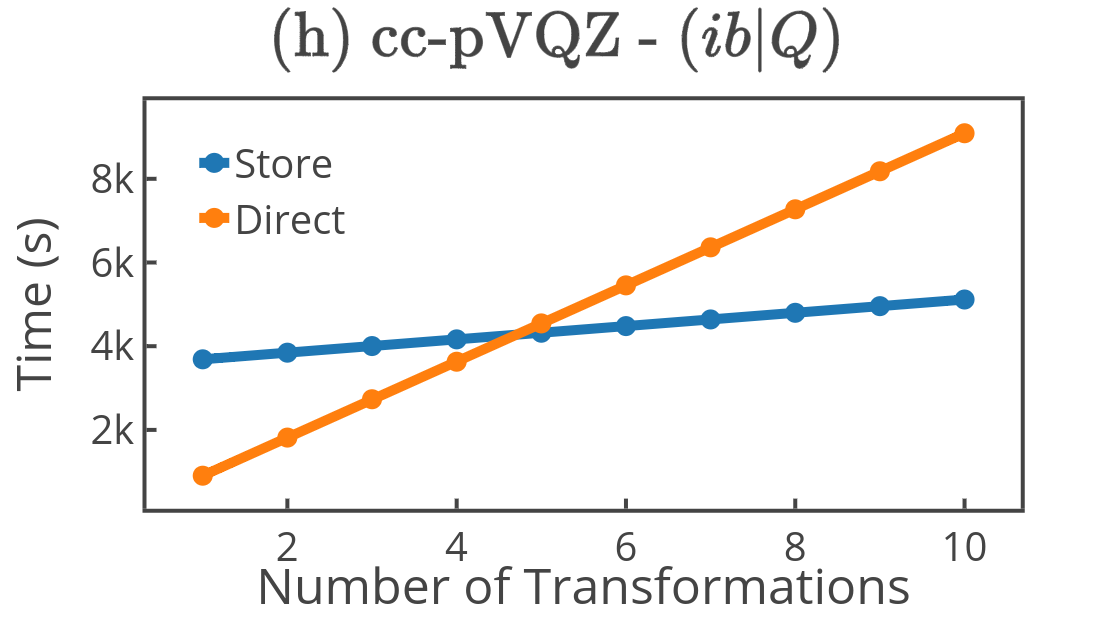
\includegraphics[width=0.35\textwidth]{figures/workflow_plots/input2-cc-pVQZ.png}}
  %\hfill
  \subfloat[]{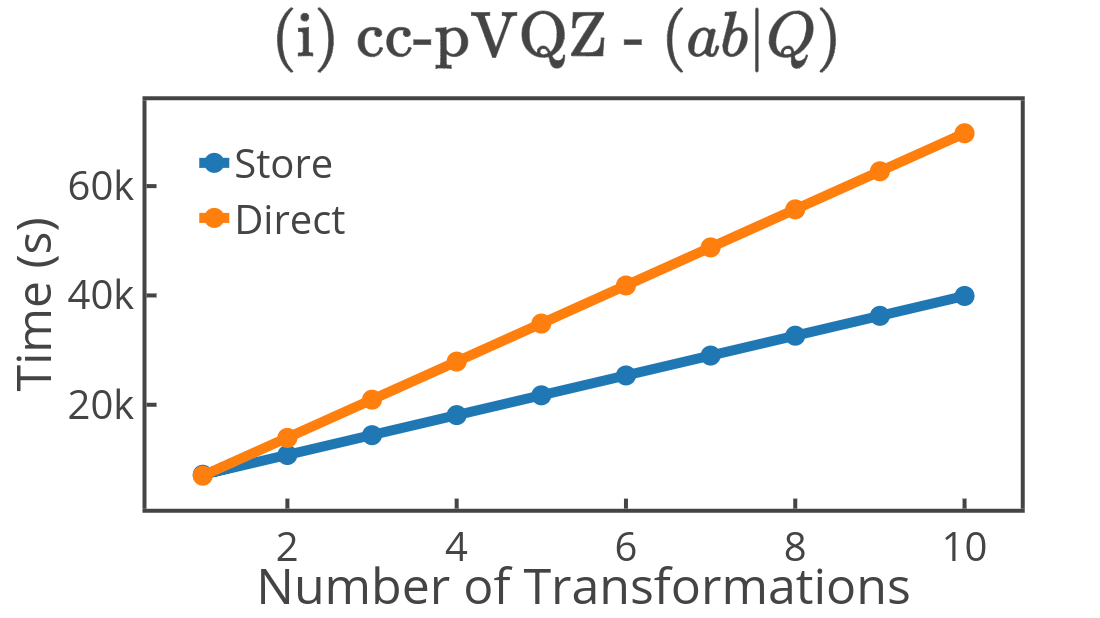
\includegraphics[width=0.35\textwidth]{figures/workflow_plots/input3-cc-pVQZ.png}}
  \caption{Comparison of execution times for the Store and Direct algorithms to complete $(ij|Q)$, $(ib|Q)$, and $(ab|Q)$ transformations
across the cc-pVDZ, cc-pVTZ, and cc-pVQZ basis sets. A scan from one to ten transformations was performed. In each case, a crossover
occurs as the Direct algorithm becomes more expensive. The crossover occurs in fewer iterations for transformations involving larger MO spaces.
With increasing basis set size, the crossover point is shifted to the right for the $(ij|Q)$ and $(ib|Q)$
transformations and it is shifted slightly to the left for the $(ab|Q)$ transformation.}
\end{figure}

If only one transformation occurs, then the speedups of Table 1 enable the Direct algorithm to be superior. 
However, the Direct algorithm must carry out expensive metric contractions for every transformation. As the
number of transformations increase, the expense of these contractions
overtakes the speedups of pre-transforming the integrals. Note that a crossover between the two algorithms occurs in each system. 
This finding supports our conjecture that the Store algorithm is advantageous in contexts where many transformations occur. 
This includes iterative methods where the transformations
are carried out in each iteration, such as MCSCF, as well as methods which require many transformations, such as FSAPT and 
USAPT. Conversely, the Direct algorithm is advantageous for methods
requiring few transformations, such as DFMP2.

Additionally, the crossover point shifts to the left as the transformation spaces get larger ($ij, ia, ab$), occuring in fewer transforamtions.
This finding is supportive of the proposed speedups in Table 1.
Therefore procedures using anything larger than a $(ib|Q)$ transformation will recieve nominal benefits from employing the 
Direct algorithm and may incur slowdowns if many transformations occur.
Last, the crossover point shifts to the right for the $(ij|Q)$ and $(ib|Q)$ transformations as larger basis sets are used. 
This will allow for 
continued benefits with more transformations. Conversely, the crossover shifts to the left for the $(ab|Q)$ transformation
for larger basis sets. Either of these findings are elucidated
by the increasing ratio of $\frac{N_{aux}}{N_{AO}}$. 
 
\subsection{Superior Workflows in Practice}

In the previous section, we determined the Direct algorithm will be superior in methods such as DFMP2, while the Store 
algorithm will be superior in methods such as MCSCF.
After determing the contexts in which either algorithm prevail, we sought to reveal their benefits when applied in practice. 
To do so, we employed either algorithm
in the contexts of different procedures and systems.  For procedures, we tested DFMCSCF and DFMP2.  We ran these 
procedures on the systems included in Figure 5.5.
Figure 5.5 (a) is a hexatriene molecule.  Figure 5.5 (b) is benzene and toluene solvated by 20 water molecules.
Table 5.5 lists the characteristics of each system,
which includes the basis set, the number of primary and auxiliary basis functions, and the mask sparsity. 


\begin{figure}[H]
  \captionsetup[subfigure]{}
  \centering
  \subfloat[]{\includegraphics[width=55mm]{geometries/hexatriene.png}}
  \subfloat[]{\includegraphics[width=55mm]{geometries/benzene-toluene-solvated.png}} 
  \hfill
  \caption{Systems used for context dependent investigation of the Store and Direct workflows. (a) Hexatriene. (b) Benzene and toluene 
in 20 water solvent molecules. }
\end{figure}

\begingroup
\begin{table}[H]
\centering
\renewcommand{\baselinestretch}{1}
\caption{Characteristics of systems for Store vs Direct algorithm comparisons.}
\begin{tabular}{l cccc}
\multicolumn{1}{l}{\textbf{System}} &
\multicolumn{1}{c}{\textbf{Basis}} &
\multicolumn{1}{c}{\textbf{$N_{aux}$}} &
\multicolumn{1}{c}{\textbf{$N_{occ}$}} &
\multicolumn{1}{c}{\textbf{$N_{virt}$}} \\
\hline
Hexatriene        & cc-pVQZ     & 3277      & 129       & 542        \\ 
Benzene-Toluene   & jun-cc-pVDZ & 3856      & 129       & 1437       \\ 
\end{tabular}
\end{table}
\endgroup

The experiments were carried out using one node consisting of an Intel Core i7-5930K processor
(6 cores at 3.50GHz) and 60GB DRAM. The results are included in Tables 5.6 and 5.7. Table 5.6 includes
the total computation time spent in operations involving the three-index integrals. These times will
reflect the algorithmic benifits illustrated in Table 5.4. Table 5.7 includes the total time required
to exectue the program. These times reflect total procedure times, which include many operations extraneous
to the three-index integrals.

\begingroup
\begin{table}[H]
\centering
\renewcommand{\baselinestretch}{1}
\caption{Computatoinal times comparing the Direct and Store algorithms for three-index integral transformations}
\begin{tabular}{l cccc}
\multicolumn{1}{l}{\textbf{System}} &
\multicolumn{1}{c}{\textbf{Procedure}} &
\multicolumn{1}{c}{\textbf{DIRECT}} &
\multicolumn{1}{c}{\textbf{STORE}} &
\multicolumn{1}{c}{\textbf{Speedup}} \\ 
\hline
Hexatriene        & DFMCSCF & 42.32s  & 7.839s  &  5.4x  \\ 
Hexatriene        & DFMP2   & 2.728s  & 6.559s  &  2.4x  \\ 
Benzene-Toluene   & DFMCSCF & 438.1s  & 104.8s  &  4.2x  \\ 
Benzene-Toluene   & DFMP2   &      &   &    \\ 
\end{tabular}
\end{table}
\endgroup


\begingroup
\begin{table}[H]
\centering
\renewcommand{\baselinestretch}{1}
\caption{Total procedure wall clock times comparing the Direct and Store algorithms for three-index integral transformations}
\begin{tabular}{l cccc}
\multicolumn{1}{l}{\textbf{System}} &
\multicolumn{1}{c}{\textbf{Procedure}} &
\multicolumn{1}{c}{\textbf{DIRECT}} &
\multicolumn{1}{c}{\textbf{STORE}} &
\multicolumn{1}{c}{\textbf{Speedup}} \\ 
\hline
Hexatriene        & DFMCSCF & 173.0   & 145.6   &  1.2x  \\ 
Hexatriene        & DFMP2   & 1299.4s & 1307.3s &  1.0x  \\ 
Benzene-Toluene   & DFMCSCF & 5138.7s & 4811.8s &  1.1x  \\ 
Benzene-Toluene   & DFMP2   &   &   &    \\ 
\end{tabular}
\end{table}
\endgroup

Both Tables 5.6 and 5.7 reveal that the Direct algorithm is superior for DFMP2 whereas the Store algorithm is superior for
DFMCSCF. The computational speedups can be substantial, reaching 5.4x for DFMCSCF with the hexatriene system. However, Table 5.7
reveals these speedups are considerably dampened for the overall procedure time. This is true because 
the operations invovling the three-index integrals ar enot the most expensive compoutations occurring within these procedures.


\section{Coloumb and Exchange Builds}

Here, we present the performance of Algorithms 10 and 11 for various systems. Currently, the state of the art in the 
open-source electronic structure package, Psi4, is Algorithm 11. However, we conjecture that Algorithm 10 could provide 
considerable speedups as it eliminates entirely a strided, level 1 BLAS copy.   

We implemented Algorithm 10 and incorporated it into a development version of Psi4. Then, we used Psi4's Self-Consistent-Field
procedure to produce energies for various systems and basis set combinations. The systems used involved a protein-drug complex,
where the drug molecule is ommitted and the atoms of the protien are added in a series according to distance from the center of
the drug molecule. 

The experiments were carried out using one node consisting of an Intel Core i7-5930K processor
(6 cores at 3.50GHz) and 60GB DRAM. The results are included in Table 5.7:


 
 

